\section{DbA Techniques Based on Creative Process}
We refer to previous work and articles related to the creative process definition\cite{frich2019mapping, chung2021intersection, hsueh2024counts, cross2021engineering, keates2002user, weaver2010transformation} to collect the techniques based on the creative process and provide corresponding cases based on corpus collection. It is worth mentioning that most of the work does not only serve one stage. The division is based on the maturity of ideas, the entire process is categorized into 4 primary stages and 7 iterative sub-processes, to emphasize the forms and contents that DbA technique can assist. At each stage, we will classify cases into three levels: Assist, Augment, and Automate, based on the degree of human-computer collaboration, and describe them accordingly. At the Assist level, the software assists with specific techniques such as screening, retrieval, and mapping to reduce cognitive load. At the Augment level, human-computer collaboration stimulates thinking and creativity. At the Automate level, the machine iterates on content independently, with humans assisting in the iteration direction.
%我们参考以往工作和creative process理论相关文章得到基于创造过程的技术分类,并基于语料库收集给出一些相应的案例。值得一提的是多数工作并不仅服务于一个阶段,加以划分只是强调类比设计可以辅助的形式和内容。在每个阶段,我们将根据人机协作的程度,将案例分为三个层级进行描述,分别是:assist、augment和automate。在assist层级软件辅助筛选、检索、映射等相关具体技术,减轻认知负荷,在augment层级人机协作相互刺激思考和创造力,automate则是机器自主迭代内容,人辅助迭代方向。

%Assist (人机筛选结合) < Augment (Co-create人机相互刺激) < Automate (机器自主迭代) 90%
\subsection{Phase 1: Problem Definition}
The core mission of this phase is to precisely define problems by revealing structural contradictions rather than initiating a design based on superficial statements\cite{simon2019sciences, hsueh2024counts} as illustrate in Fig \ref{fig:Create Process}. Defining the design problem confronts three dilemmas: (1) Arbitrary starting points risk solution-target misalignment and resource waste. (2) When existing solutions fail to resolve issue. For example, in 1996, the Brazilian policy was hindered by the lack of basic data and interface design\cite{barzelay2007learning}, it is necessary to identify the real pain points. This process relies on interdisciplinary experience, and those without experience are difficult to be competent. At this time, DbA can assist in attribution and the transfer of indirect experience. (3) Entrenched traditional methods often compel visionary designers to compromise with classical cases\cite{wills1994towards}. We use the metaphor of standing under the wall and cannot see the landscape outside the wall to represent the dilemma in \textit{Vision} phase and standing on the information and experience provided by DbA system will get into the \textit{Inspiration} phase in Fig.\ref{fig:Create Process}. Integrating DbA assists in problem definition can through content tracing and inference while expanding conceptual horizons\cite{hewstone1990ultimate}, assisting designers to internalize visions and missions, providing the possibility to solve the problem mentioned above. The technological content processed at this stage is diverse, fragmented, distributed across domains, and governed by ambiguous logic\cite{li2010agentsinternational}.
%此阶段创造任务的核心在于精准定义问题本质、揭示结构性矛盾,而非基于表面陈述直接设计。定义设计问题面临三重困境:首先,武断的起点易导致方案偏离目标并引发资源浪费;其次,当既有方案无法解决问题时(如1996年巴西政策因基础数据与交互设计缺失受阻),需识别真实痛点,该过程依赖数据采集与界面设计经验,无经验者难以胜任,此时类比设计可辅助归因与间接经验传递;最后,传统方法的根深蒂固常迫使前瞻性设计师妥协于经典案例。引入类比设计,能通过深度溯源与因果推断准确定义问题,同时提供开阔思路,帮助设计师内化愿景和任务,为解决上述困境提供可能。此阶段的技术所处理的内容是多元碎片化的、跨领域分布的、模糊逻辑的。

\textbf{\underline{Vision.}} Technology at this stage aims to provide artistic inspiration and visionary support for those with vague problems, such as market and user research, risk prediction and etc. At the \textit{Assist} level, within the decision-making contexts of software feature development, Zhang et al. employs DbA theory based recommendation techniques for similar product features to conduct user research and infer development directions\cite{zhang2017systematic}. Similarly, He et al. utilize multi-modal technologies to mine and characterize existing case libraries for assisted directional ideation for future transportation system design\cite{he2019mining}. At the \textit{Augment} level, during preliminary market observation and decision formulation in international investment, Li et al. propose a multi-agent integrated decision support application that leverages knowledge bases, simulations, and fuzzy logic to enhance investment direction forecasting\cite{li2010agentsinternational}. Concurrently, in creative design, researches have shown that collaborators with different cognitive depths in problem articulation can inspire participants and AI robots to construct multiple visions for the same problem\cite{yu2014distributed, chan2014conceptual, christensen2016creative}. At the \textit{Automate }level, scenarios applied DbA methods to generate heuristic direction, such as using topic modeling firm management assessment for policy strategy\cite{gavetti2005strategy}, defining specific problem for service design\cite{moreno2014analogies}.
%此阶段的技术旨在为那些面临模糊问题(如市场/用户调研、风险预测等)的人提供艺术灵感和前瞻性支持。 在辅助(Assist)层级,软件功能开发决策的研究中,文献 【19】采用基于设计知识库(DbA)理论的相似产品功能推荐技术执行用户调研并推导开发方向;类似地,文献 【68】通过多模态技术挖掘与表征案例库以支持定向交通系统规划构思。在增强(Augment)层级,国际投资理财领域的前期决策阶段,文献 【84】开发了集成多智能体的决策辅助应用,结合知识库、模拟推演及模糊逻辑提升投资方向预判能力;创意设计领域的研究 【5,33,69】则表明,不同认知深度的合作者阐述问题可激发参与者/机器对同一问题的多元愿景建构。在自动化(Automate)层级,诸如使用主题建模的企业管理评估【79】、服务设计问题定义【76】等场景有很多工作已应用DbA方法来生成启发式方向。


\textbf{\underline{Inspiration.}} It refers to the assistance in inspiration stimuli and design heuristics through DbA techniques. Research at this stage demonstrates diversified technical approaches. At the \textit{Assist} level, Zhu et al. extract bioTRIZ inspired innovation stimuli through functional case modeling of biological functions\cite{zhu2023design}. Emuna et al. use semantic retrieval and reasoning models to build a search engine for mining biological-analogical design inspiration from websites\cite{emuna2024imitation}. Murphy et al. employ the vector approach and hybrid model to search for inspiration\cite{murphy2014function}, and Moreno et al. utilize the rule-based case library for the retrieve and generate of solutions\cite{moreno2014fundamental}. \textit{AskNatureNet} further facilitates the divergent thinking to stimulate inspiration through structured knowledge visualization\cite{chen2024asknaturenet}. At the \textit{Augment} level, \textit{AnalogiLead} enables linguistic chunk and recombination via interaction design for perceiving more analogy ideas\cite{srinivasan2024improving}, and Kang et al. integrate several resource platforms to trigger inspiration through visual and text stimuli\cite{kang2025biospark}. \textit{AnalogyMate} confirms textual prompts stimulate proportional data reflection\cite{chen2024beyond}, whereas \textit{BIDTrainer} enhances knowledge acquisition via structured interfaces\cite{chen2024BIDTrain}. At the \textit{Automate} level, \textit{STORYANALOGY} leverages large language models to mine and generate narrative-level creative analogies\cite{jiayang2023storyanalogy}, Warner et al. use the interactive flexible method to achieve direct cross-domain style transfer\cite{warner2023interactive}, and \textit{VASR} method accomplish context-aware analogical image recognition and synthesis\cite{bitton2023vasr}.
%指的是通过DbA技术在灵感激发和设计启发方面提供的帮助。该阶段研究呈现多维技术路径分化:在辅助(Assist)层级,Zhu等人 [57]基于功能案例建模从生物效应角度提取BioTRIZ创新启发,等人使用语义搜索和推理模型构建了从网络挖掘生物类比设计灵感搜索引擎[24],Murphy等 [53]采用混合模型搜索类比灵感,Fu等人 [40]运用规则驱动的案例库检索生成方案,而AskNatureNet [38]则通过仿生知识可视化引导发散思维;在增强(Augment)层级,研究 [1]利用交互设计实现类比组块重组,文献 [2]借助资源网站推荐系统触发生物类比联想,[10]证实文字提示可激发数据比例反思,BIDTrainer [7]则通过结构化界面促进新知吸收;在自动化(Automate)层级,STORYANALOGY [16]依托大语言模型挖掘叙事级创意类比,方法 [9]实现跨领域风格映射的直接生成,VASR等系统则完成情境化类比图像的识别与合成,



\subsection{Phase 2: Product Ideation}

The core objective of this phase is to derive a feasible design solution based on the prior definition of the problem and exploratory analysis. As the ideation phase commits around 80\% of the project costs, its quality of decision-making critically determines the performance of the sustainability of the product\cite{kerzner2025project}. Research indicates that Design-by-Analogy (DbA) systems effectively mitigate resource waste and overcome design fixation through each stage of it's procedure\cite{o2015toward}. By integrating domain knowledge data\cite{jiang2022data} and experience repositories, this approach automates the abstraction of source problem and the generation of the target solution, producing innovations characterized by convergence, goal-oriented, and deep integration of user needs\cite{fu2015design}. During transition between the sub-process, such as from ideation to prototype, DbA can assist structural refinement of a certain framework, aesthetic enhancement of the overall appearance and scheme polishing of the transactional work.
%本阶段的核心任务是根据前期的问题定义和相关探索得出一个可行的设计方案。设计构思阶段作为锁定80%项目成本的核心环节,其决策质量直接影响商品可持续性表现\cite{kerzner2025project}。研究表明,基于智能类比设计(Design-by-Analogy, DbA)的系统可通过编码-检索-映射-评估机制,结合领域知识库与模糊经验库实现源域问题抽象化及目标域方案生成,有效规避资源浪费并突破设计固定效应。该方法产出方案兼具收敛性、目标聚焦性及用户深层需求融合性。在从构思过渡到原型的过程中,基于类比设计(DbA)可辅助结构优化、美学提升和方案完善。事务性工作


\textbf{\underline{Ideation.}} Distinct from inspiration, this phase involves design convergence, where DbA technology assists users in synthesizing multiple inspirations into ideas. At the \textit{Assist} level: Kim et al. employ Bayesian case-based modeling for prototype generation\cite{kim2014bayesian}. Han et al. develop generative computational tools using 16 ontologies with image and knowledge databases\cite{han2018computational}. Bitton et al. construct visual analogy datasets through situation recognition annotation and CLIP models\cite{bitton2023vasr}. He et al. achieve directed design convergence through conceptual space mining\cite{he2019mining}. Luo et al. stimulate design ideation by regulating knowledge distance\cite{luo2021guiding}. Chen et al. assist ideation leverage semantic-visual combinatorial models\cite{chen2019artificial}and other techniques\cite{akula2023metaclue, you2018design, shen2022nature}. At the \textit{Augment} level: \textit{Pedagogical Prism} implements domain isomorphic analogies\cite{bettin2023pedagogical}. \textit{EmoSync} enables personalized empathy using affective reasoning\cite{Ju2025toward}. \textit{BioSpark} provides interactive analogy suggestions to help the idea mature\cite{kang2025biospark}. \textit{VISION} facilitates inspiration generation and integration through patent visualization\cite{song2020exploration}. At the \textit{Automate} level: Zhai et al. leverage case-based methods autonomously mapping executes irrigation scheduling in viticulture\cite{zhai2020applying}. Caley et al. applied a retrosynthesis prediction algorithm and robotic workflow to automate the synthesis of organic compounds\cite{coley2019robotic}. Moreover, Zhang et al. implemented the autonomous decision making module for intelligent process planning for digital twin manufacturing cells (DTMC) based on deep learning\cite{zhang2020deep}.
%区别于inspiration,这一阶段包含思维的收敛,指的是通过DbA技术辅助用户将众多灵感收敛成为一个新的idea。
%在辅助(Assist)层级,kim等人使用贝叶斯案例模型基于案例和原型进行生成【6】,han等人开发了基于16种本体和图像、知识数据库进行类比推理的生成式计算工具【45】,Bitton等人使用情景识别注释和CLIP模型构建了大规模候选类比数据集用于识别和生成情境类比【18】,He等人【68】通过概念空间挖掘与表征实现定向创意构思,Luo等人通过调整知识距离引导数据表证从而激发设计思考【41】,chen等人通过语义构思网络和视觉概念组合模型辅助构思【54】,其他种类技术【25,72,47】
%在增强(Augment)层级,Pedagogical Prism将领域同构类比作为计算机教育中的启发【48】,基于微侵犯情境,ju等人使用情感推理和内容生成辅助个性化共情【49】,BioSpark通过生成和交互辅助用户完成类比构思并给出建议【2】,VISION 则通过可视化专利知识库促进灵感交互生成【71】
%在自动化(Automate)层级,【12】葡萄种植中的灌溉调度,在基于学习机制的机器上根据案例检索和当前状态自主完成映射,inkspire通过类比草图迁移辅助设计概念探索和完善【50】,【80】使用基于案例的自动规划有机化合物流动合成平台,【81】zhang等人基于深度学习实现数字孪生制造单元(DMTC)的智能工艺规划.


\textbf{\underline{Prototype.}} This phase involves DbA technology that assists users in refining, upgrading, and iterating predefined ideas. At the \textit{Assist} level: \textit{Textoshop} adopts image editing logic for textual Boolean operations\cite{masson2025textoshop}. Dimassi et al. recommend multimaterial knowledge through semantic similarity vectors to  faclitate intelligent 4D printing\cite{dimassi2023knowledge}. In addition, Liu et al. employ SMFM-based tools enable similar product details retrieval for prototypes\cite{liu2023smfm}. At the \textit{Augment} level: \textit{Umitaton} extracts and edits user-interface(UI) response behaviors for front-end development projects\cite{chen2021umitation}. \textit{InnoGPS} visualizes patent databases for innovation recommendations\cite{luo2019computer}. Moreover, \textit{Xcreation} generates narrative illustration prototypes through cross-modal generation\cite{yan2023xcreation}. At the \textit{Automate} level: Fischer et al. accomplish autonomous 3D attributes analogical transfer  leverage NeRF method\cite{fischer2024nerf}. Zhang et al. achieve 2D visual analogy transfer using CNN and hierarchical GCN\cite{jin2022visual}. \textit{Toontalker} implements facial animation re-targeting with Transformer architectures\cite{gong2023toontalker}.
%这一阶段指的是dba技术帮助用户围绕一个预设好的idea进行打磨,升级和迭代。
%在辅助(Assist)层级,Textoshop利用图片编辑的逻辑迭代文字编辑,如对文本片段进行布尔运算以构建更复杂的文本【4】,Dimassi等人基于语义相似性向量空间为多材料4d打印推荐知识【63】,基于smfm的产品检索推荐工具【61】,
%在增强(Augment)层级,【32】umitation提取、编辑目标网站的ui行为并将其应用于设计项目,【62】InnoGPS开发基于云的专利库可视化检索工具为专利推荐创新,Xcreation基于图文跨模态生成叙事插画原型【15】
%在自动化(Automate)层级,fischer等人基于神经辐射场nerf迁移示例3d模型的属性【20】,zhang等人基于卷积神经网络(CNN)和层次结构的图卷积网络(HGCN)将学习到的视觉知识实现视觉类比迁移和生成【74】,toontalker基于transformer实现人脸动画的重演原型【27】



\subsection{Phase 3: Product Implementation} 
This phase focuses on the implementation of a certain idea with its finalized basic logic, tangible output, and standardized production. Although DbA methodologies are predominantly applied to early-stage creative research and it's efficiency is obvious, a few work focus on the implementation of fabrication phase of DbA. This phenomenon reveals an epistemological gap between the implementation of DbA methods in practical operational techniques: The practical operational experience with strong discreteness and case specificity is difficult to be transformed into structured knowledge\cite{rigaud2022exploring}. This gap lead to the neglects of relevant experiential and embodiment data: replicable techniques\cite{schulz2014design}, niche manufacturing practices\cite{scopigno2017digital}, and embodied cultural knowledge\cite{vaisey2009motivation} face erosion without quantitative documentation. Consequently, the transfer of manufacturing experience based on DbA remains underexplored. We argue that DbA has significant potential here: In intelligent manufacturing, as long as automated production lines leverage computable material processing, where DbA-based cross-domain mapping can balance fabrication creativity and accuracy through controllable structural transfers\cite{schulz2014design}. As for cultural preservation, niche craftsmanship requires digitization through standardized parameters, transforming tacit knowledge into living repositories, where DbA can play the essence technique role for preserving and enlivenment through it's unique technology mediation nature\cite{scopigno2017digital, jiang2022data}.
%本阶段创意任务的核心是围绕具体方案实施操作、产出落地及标准化生产。类比设计领域普遍将类比设计方法用于创造前期研究,同时,制造研究者普遍关注具体的实操阶段的技术,这中间存在认知论gap,即,强离散性与案例特异性的实践操作经验难以转化为结构化知识。这一认知导致相关经验数据被忽视——可复现工艺技术、小众制造实践与具身化文化知识因缺乏量化记录而面临消亡。因此,DbA驱动的制造业经验传递成为研究洼地。我们认为DbA在此具有巨大潜力:智能制造中,只要自动化产线依赖可计算材料处理,那么基于DbA的跨领域映射就可以通过可控结构迁移平衡制造创造力与准确性。至于文化保护,小众工艺需要通过标准化参数实现数字化,将隐性知识转化为活态知识库,在这方面,基于数据的类比(DbA)可以凭借其独特的技术中介性质,发挥关键技术作用,实现文化的保护与传承\cite{scopigno2017digital, jiang2022data}。 


\textbf{\underline{Fabrication.}}
This phase covers manufacturing, development, production, and deployment, where DbA technologies enhance user implementation. At the \textit{Assist} level, You et al.'s geotechnical decision supporting system with embedded craft data\cite{you2018design}can help making detailed implementation decision. Jin et al. leverage deep learning assisted buckling-guided assembly design for 3D frame structures producing\cite{jin2023deep}, and other mentioned manufacturing assistance techniques\cite{hong2024fishbone, dimassi2023knowledge, yu2014adaptive} share the same logic. The \textit{Augment} level, \textit{Anther} applies cross-domain video tutorial retrieval for transfer of niche craftsmanship techniques
\cite{emerson2024anther}. In addition, Schulz et la. develope a system which can design,assembly and manufacturing 3d products making using example data base \cite{schulz2014design}. Riguad et al. 's robotic system are able to collect craft data automatically in niche workshops for experience recommendation\cite{rigaud2022exploring}, and Khosravani et al. deploy knowledge-based DbA methods for injection molding lines in the intelligent processing machine\cite{khosravani2022intelligent}. At the \textit{Automate} level, Zhai et al.'s case based reasoning system for agricultural irrigation can be embeded in smart city and grid infrastructures\cite{zhai2020applying}. Moreover, An et al.'s BIM-based automated manufacturability checking for wood frames\cite{an2020bim}, and automated decision support systems\cite{gonzalez2018energy, zhang2020deep, lupiani2017monitoring}are categorized in our work as facilitating fabrication phase.
%这一阶段则包含了实际的制造、开发、制作、部署等,该阶段的dba技术可以增强用户的实施操作。
%在辅助(Assist)层级,You等人基于内置制造技艺数据的岩土工程决策支持系统【72】,基于深度学习辅助三维框架结构力学组装设计【86】,相似的前文提到过的【56】【63】【65】也涉及到制造辅助
%在增强(Augment)层级,anther实现基于跨领域同制作工艺和概念的视频制造教程检索【3】,基于可制造产品数据库进行组装,拼接,设计和制造【52】,rigaud等人在小众制造工坊中部署自动化采集制造技艺技术并致力于未来经验推荐【59】,在智能制造的注塑工艺生产线中加入基于知识库的dba方法辅助【67】。
%在自动化(Automate)层级,zhai等人开发了可在智慧城市和智能电网中内嵌的农业灌溉类比推理系统【12】,基于建筑信息模型(BIM)的木框架组件可自动化制造性检查决策支持系统【78】,以及前文提到过的【82,81,85,】


\subsection{Phase 4: Product Evaluation} This phase focuses on monitoring and evaluating the life cycle of a product performance, leveraging different metrics, user feedback, risks, market response, projected outcome, and relevant policies to enable optimization, prevention, alerting, communication, and maintenance for a better product\cite{moreno2014fundamental}. Many products lack production evaluation and analysis over life cycle, resulting in many aspects being considered and implemented only after deployment.\cite{zhong2017intelligent}. DbA techniques can facilitate concurrent sustainability evaluation of product during development through data-driven case analysis and fuzzy logic assessment, enhancing holistic product sustainability\cite{liao2021priming}.
%这一阶段,创意工作的主要目标是检测和评估产品的全链路上的各项性能指标、用户反馈、风险、市场反响、预期结果、涉及到的政策等加以优化、预防、警示、传达、维修等。很多产品缺少全链路的生产评估和分析,导致许多内容是在全面部署后才开始思考和执行. 类比设计可以在开发阶段同时根据数据、案例、模糊逻辑评估设计,促进产品可持续发展。

\textbf{\underline{Evaluation.}} This phase enables DbA technologies to evaluate, predict and provide critiques, feedback and suggestions on previously completed designs. At the \textit{Assist} level, Arditi et al. predict the result of construction litigation using case data \cite{dougan2022predicting}, \textit{CAM} employs evaluation functions to assess the quality of creative analogy\cite{bhavya2023cam}, Boteanu et al. interpret analogy meanings and questions through semantic networks\cite{boteanu2015solving}, and Hill et al. evaluate analogy making precision through contrasting abstract relational structures\cite{hill2019learning}. At the \textit{Augment} level, \textit{BioSpark} automatically generates solution recommendations and feedback for an idea\cite{kang2025biospark}, \textit{Anther} computes conceptual distance and ``concept gravity'' scores to evaluate analogies similarity between different  niche fabrication \cite{emerson2024anther}. Moreover, Malone et al. forecast the distribution of profit and equity in supply networks through contest network design \cite{malone2017putting}. At the \textit{Automate} level, Thomas et al. extend and automate the optimization and generation of maintenance requirementss for software and mechanical systems using system theoretic hazards analysis (STHA)\cite{thomas2013extending}, An et al. conduct automated manufacturability checks\cite{an2020bim} , with similar approaches applied in\cite{coley2019robotic, zhang2020deep, gonzalez2018energy}.
%这一阶段的dba技术可以评估,预测,建议,反馈前期已经完成的设计。
%在辅助(Assist)层级,基于案例数据预测建筑工程诉讼结果【14】,cam使用评估函数评估创意类比的质量【16】,使用语义网络解释类比问题【23】,通过对比抽象关系结构评估类比制作【29】。
%在增强(Augment)层级,Biospark系统自动提供方案的建议和反馈【2】,anther通过计算评估概念距离和concept gravity score来评估类比【3】,通过竞赛网络设计实现根据供应网络的利润和股权分配的预估【34】
%在自动化(Automate)层级,
%【77】Thomas等人基于系统理论危害分析,扩展和自动化软件和机械的优化、维修等需求的生成与分析,【78】an等人进行自动化可制造性检查,相似的还有【80,81,82】

\textbf{\underline{Meta.}}
This phase enables DbA technologies to facilitate global management of design processes. At the \textit{Assist} level, Andriani et al. argue that using mapping method can facilitate end-to-end perfume production workflows transfer to global practices in wine-making provide an example for automation the supply chain migration\cite{andriani2025perfume}, similar examples as shown in\cite{you2018design, song2020exploration}. At the \textit{Augment} level, Cao et al.'s analogy tool support interdisciplinary collaboration between AI researchers and medical specialists for their overall communication and terminology translation\cite{cao2025medai}, while \textit{Analogies to Succeed} employs global transactional workflows mapping and transfer to support service design management\cite{moreno2014analogies}, similar example\cite{karunathilaka2025intuit, wills1994towards, bettin2023pedagogical, li2010agentsinternational}. At the \textit{Automate} level, Thomas et al. extract future iteration requirements for a product across both software and mechanical development processes data set to support global design practices\cite{thomas2013extending}, similar example\cite{yu2016distributed, bitton2023vasr, lupiani2017monitoring}.
%这一阶段的dba技术致力于全局管理整个设计。%在辅助(Assist)层级,将香水生产的全链路映射到酿酒制造产业的全局实践【66】供应链迁移
%在增强(Augment)层级,类比工具辅助人工智能研究员和医学专家之间的跨学科全局交流合作【39】,Analogies to Succeed使用管理服务设计问题中的全局事务性工作【76】,
%在自动化(Automate)层级,thomas等人从软件和机械开发的各个流程中提取需求辅助全局的设计实践【77】,


\begin{figure}
    \centering
    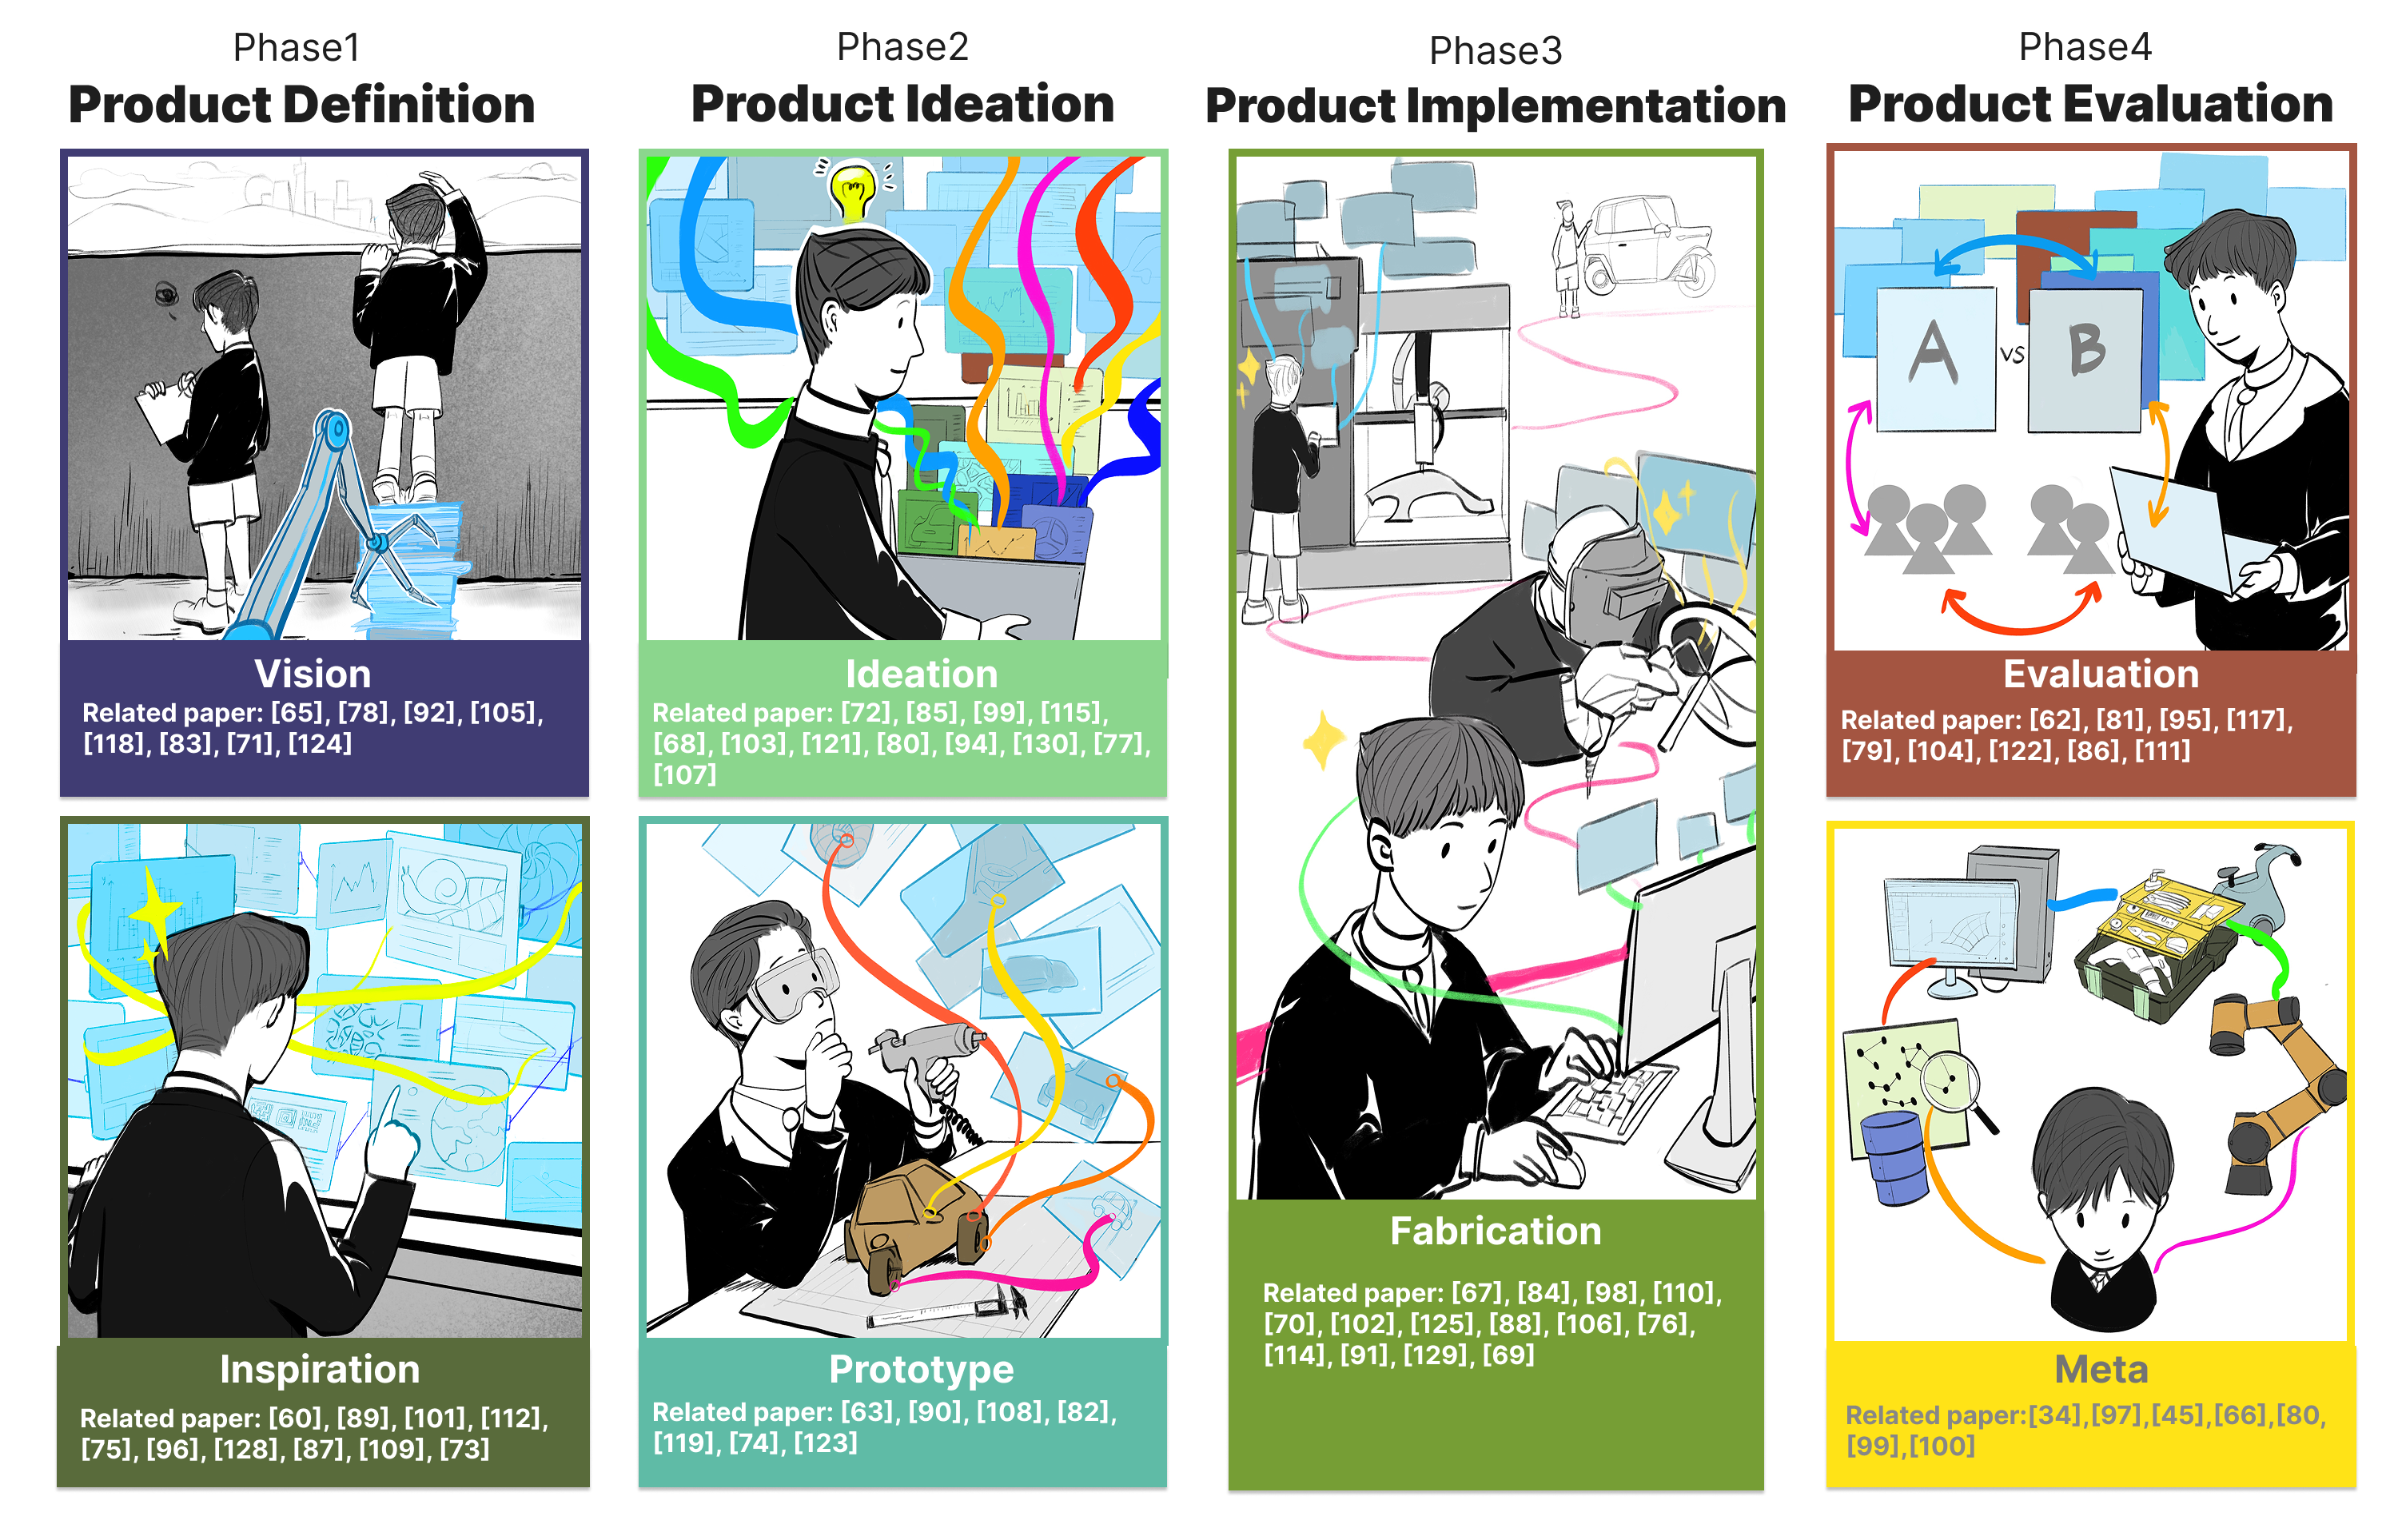
\includegraphics[width=1\linewidth]{Figures/CreateProcess.png}
    \caption{To elaborate on the technical mediation value\cite{smits2019values} of Design-by-Analogy (DbA) across different segments, we employ comic illustrations to visualize its abstract functions throughout various design phases. Based on the maturity of ideas, the entire process is categorized into 4 primary stages and 7 iterative sub-processes: in \textbf{\textit{Vision}}, the illustration adopts a metaphor where individuals standing behind a wall are unable to perceive distant landscapes, symbolizing that DbA can act as a knowledge-based foundation to elevate human cognitive horizons. In \textbf{\textit{Inspiration}}, it portrays that those positioned at a sufficient height can access diverse sources of inspirational stimuli. In \textbf{\textit{Ideation}}, DbA facilitates the screening of multiple inspirational stimuli and guides operators to independently converge heterogeneous stimuli into a coherent idea. In \textit{\textbf{Prototype}}, DbA recommends professional practices to support the optimization of ideas. In \textit{\textbf{Fabrication}}, DbA technology can be integrated into relevant software and hardware systems to provide experiential assistance and knowledge transfer for specific operational processes. And both \textbf{Evaluation} and \textbf{\textit{Meta}} stage are designed to assist operators in achieving experiential migration.}
    \label{fig:Create Process}
\end{figure}





%我们用漫画插图的形式表达每个部分DbA技术可以起到的技术中介价值,展现了在各个设计阶段,Design-by-Analogy技术可以起到的抽象作用。按照idea的成熟度,我们划分了四个主要阶段和迭代的7个子过程。其中vision阶段,插图使用站在墙后无法看到远处风景的隐喻,暗示dba可以作为垫起人类认知视野的知识地基,inspiration阶段,站的足够高的人可以接触多样化的灵感刺激,ideation阶段则是dba辅助人类对多种灵感刺激进行筛选,引导操作者自主将多类型的刺激收敛为一个idea,prototype阶段,dba则推荐更多专业做法辅助优化idea,fabrication阶段,dba技术可以嵌入在相关软件和硬件中对具体实操进行经验辅助和迁移,evaluation阶段和meta阶段也将辅助操作者进行经验迁移。




















%---------------------draft---------



%1.这一阶段,创意任务的主要内涵是定义问题,发现真正的结构性问题所在,而非有一个statement就直接开始设计,新的设计挑战往往面临:(1)武断的设计出发点会导致设计结果偏离初始目标,也会导致经济和投资的亏空和损失,本阶段可以设计师在设计前期节省成本、深刻溯源及因果推断。(2)所需产品或设计已经有其他人进行开发和解决了,找到真正的痛点问题才能真的解决问题,比如在这一设计研究中xxx得到证实,大约有xx的社区纠纷的主要矛盾并非人与人,而是环境设计的问题,这样的归因链路仰赖丰富的环境设计经验和人类学经验,是很难被没有设计背景的任意学科工程师所找到的,这就需要相关的领域知识经验库。(3)在启发阶段,类比设计可以提供更开阔的思路,更加全面的语料库检索,打开用户的思路,xxx证明会有启发帮助能力,这个阶段的内容会是多样的,零散的,分布在多个远距离领域尚未聚焦的状态,是混沌的但是充满可能性的,未经用户的内在知识运作的。

%2.研究表明,80%的设计成本在构思阶段即被锁定。大量商品耗材、能源浪费及不可持续性设计产物(如无效设计与废弃方案),可借由经验体系与智能类比设计系统辅助在本阶段规避。DbA通过「问题定义-启发收敛」框架支持用户生成完整方案,该方案具有收敛性、目标聚焦性,且深度融合用户内在经验与核心需求。至原型阶段,用户可对特定方案进行深度迭代优化(如结构修正、流程改进、美学升级),系统将启动领域适配型类比推荐机制,提供近距离参考案例的细节处理技巧、失效预防策略及领域知识迁移路径,支撑方案的精细化打磨。



%3.这一阶段,创意任务的主要内涵是围绕着某一具体想法进行实际的操作、落地产出和标准化生产。市面上观点认为类比或基于认知的方法仅仅只能在创造阶段的前期进行辅助,这一观点暗含一种假设,即,致力于研究物理制造的研究者们默认在实际操作阶段的经验难以或不能被转化成结构化的知识,因为具体操作阶段往往是case by case的,其个性和特异性较大。这一认识潜在造成了许多经验化的操作流程的数据的根本性模糊,如,本可以被大范围复现的实操工艺,小众制造技艺及实践文化,被从制造者的经验上和认知上不加以定量记录,模糊记录或者不认为可以定量记录的手工实操中遭遇忽略甚至遗失。所以基于类比设计的制造阶段的经验转移可以说是一个尚未被大面积开发的研究领域,时常被急于落地的制造者们主动忽略。我们认为在此阶段类比设计方法有着大量潜力。因为自动化的,标准化的执行和生产在流水线中基本完全仰赖大型智能制造机械,只要耗材经过可被计算的软件和机器进行生产,那么就可以被经由可推理,可结构化映射的类比设计方法增强设计决策和创造力。同时,小众的手艺和文化的传承也仰赖标准化,精确的制造参数和工艺流程来进行记录和传承,这些经验是文化档案,也是可被迁移和转化用于新的设计的类比设计所需数据。




% \textbf{\underline{Production.}}
% %这一阶段与上一阶段不具有清晰的界限,更偏向于投入流水线之后的具体操作,本阶段使用类比设计技术的全流程整合可以辅助用户实现自动化的操作。

